%%%%%%%%%%%%%%%%%%%%%%%%%%%%%%%%%%%%%%%%%%%%%%%%%%%%%%%%%%%%%%%%%%%
%TO AVOID FORMATTING ISSUES, COMPILE THIS ONLY AT WWW.OVERLEAF.COM%
%%%%%%%%%%%%%%%%%%%%%%%%%%%%%%%%%%%%%%%%%%%%%%%%%%%%%%%%%%%%%%%%%%%

%%%%%%%%%%%%%%%%%%%%%%%%%%%%%%%%%%%%%%%%%%%%%%%%%%%%%%%%%%%%%%%%%%%
\documentclass[a4paper,12pt]{article}
\usepackage{graphicx}
\usepackage{subfig}
%To use this font, you need XeTex or LuaTex, prefer openleaf
\newenvironment{codefont}{\fontfamily{ccr}\selectfont}{\par}

\title{
	\normalfont \normalsize 
	\textsc{Pimpri Chinchwad College of Engineering \\ 
		Computer Laboratory - IV} \\
	[10pt] 
	\rule{\linewidth}{0.5pt} \\[6pt] 
	\huge Assignment No - A3 \\
	\rule{\linewidth}{2pt}  \\[10pt]
}
\author{}
\date{\normalsize}


\begin{document}
\maketitle

%%%%%%%%%%%%%%%%%%%%%%%
% FOR A NUMBERED LIST
% \begin{enumerate}
% \item Your_Item
% \end{enumerate}
%%%%%%%%%%%%%%%%%%%%%%%
% FOR A BULLETED LIST
% \begin{itemize}
% \item Your_Item
% \end{itemize}
%%%%%%%%%%%%%%%%%%%%%%%
% TO IMPORT AN IMAGE
% \includegraphics[width=\textwidth]{name_of_file}
% \textwidth makes the picture the width of the paragraphs
%%%%%%%%%%%%%%%%%%%%%%%%%%%%%%
% TO CREATE A FIGURE WITH A NUMBER AND CAPTION
% \begin{figure}
% \includegraphics[width=\textwidth]{image}
% \caption{Your Caption Goes Here}
% \label{your_label}
% \end{figure}
% REFER TO YOUR FIGURE LATER WITH
% \ref{your_label}
% LABELS NEED TO BE ONE WORD
%%%%%%%%%%%%%%%%%%%%%%%%%%%%%
% TO ADD CODE
% \begin{codefont}
% Some code in "courier" font
%\end{codefont}
%%%%%%%%%%%%%%%%%%%%%%%%%%%%%
\section{Aim}
	\paragraph{} A Web Tool for Booth’s multiplication algorithm is used to multiply two numbers located in distributed
	environment. Use software design client-server architecture and principles for dynamic programming.
	Perform Risk Analysis. Implement the design using HTML-5/Scala/ Python/Java/C++/ Rubi on Rails.
	Perform Positive and Negative testing. Use latest open source software modeling, Designing and testing
	tool/Scrum-it/KADOS and Camel.
	
\section{Objective}
	\begin{itemize}
		\item To perform booth's multiplication
	\end{itemize}
	
\section{Software Requirements}
	\begin{itemize}
		\item	Linux Operating System
		\item	GCC
		\item	Umbrello
	\end{itemize}
	
\section{Mathematical Model}
	\paragraph{} \
	S= {s, e, X, Y, Fn, DD, NDD}\\
	Where, \\
	s = Initial State\\ 
	e = End State \\
	X = Input : Two numbers to be multiplied\\
	Y = Output : Multiplication of integers\\
	Fn = Function used in program\\
	DD=Deterministic Data \\
	NDD = Nondeterministic Data\\ 
	
\section{Theory}
	\subsection{Client server model}
		\paragraph{} The Client-server characteristic describes the relationship of cooperating programs in an application. The server component provides a function or service to one or many clients, which initiate requests for such services.
		\paragraph{}Servers are classified by the services they provide. For instance, a web server serves web pages and a file server serves computer files. A shared resource may be any of the server computer's software and electronic components, from programs and data to processors and storage devices. The sharing of resources of a server constitute a service.
		\paragraph{} Whether a computer is a client, a server, or both, is determined by the nature of the application that requires the service functions. For example, a single computer can run web server and file server software at the same time to serve different data to clients making different kinds of requests. Client software can also communicate with server software within the same computer.Communication between servers, such as to synchronize data, is sometimes called inter-server or server-to-server communication.
		
		\begin{figure}[htb!]
			\centering
			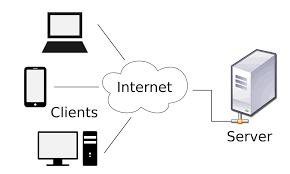
\includegraphics{images.png}
			\caption{Client Server Model}
			\label{Client Server Model}
		\end{figure}
		
	\subsection{Client Server Communication:}
		\paragraph{} In general, a service is an abstraction of computer resources and a client does not have to be concerned with how the server performs while fulfilling the request and delivering the response. The client only has to understand the response based on the well-known application protocol, i.e. the content and the formatting of the data for the requested service.
		\paragraph{} Clients and servers exchange messages in a request–response messaging pattern: The client sends a request, and the server returns a response. This exchange of messages is an example of inter-process communication. To communicate, the computers must have a common language, and they must follow rules so that both the client and the server know what to expect. The language and rules of communication are defined in a communications protocol. All client-server protocols operate in the application layer. The application-layer protocol defines the basic patterns of the dialogue. To formalize the data exchange even further, the server may implement an API (such as a web service). The API is an abstraction layer for such resources as databases and custom software. By restricting communication to a specific content format, it facilitates parsing. By abstracting access, it facilitates cross-platform data exchange.
		\paragraph{} A server may receive requests from many different clients in a very short period of time. Because the computer can perform a limited number of tasks at any moment, it relies on a scheduling system to prioritize incoming requests from clients in order to accommodate them all in turn. To prevent abuse and maximize uptime, the server's software limits how a client can use the server's resources. Even so, a server is not immune from abuse. 



\subsection{Booth's Algorithm flow chart}
		\begin{figure}[h!]
			\centering
			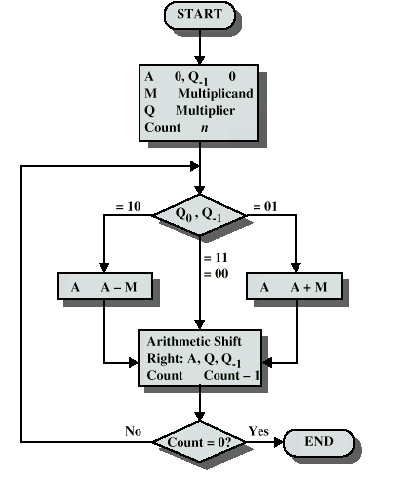
\includegraphics[scale=0.60]{booth}
			\caption{Booth's Multiplication Flowchart}
			%\label{Booth's Multiplication Flowchart}
			
			\end{figure}

			\begin{figure}[htb]
			
			\centering
			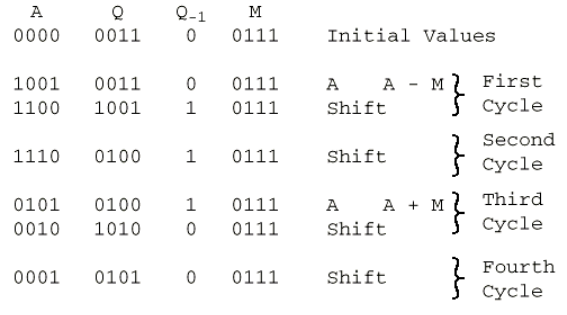
\includegraphics[scale = 0.60]{boothex}
			\caption{ Multiplication (7*3) using Booths Algorithm}
			%\label{Booth's Multiplication Flowchart}
		\end{figure}
\newpage

\subsection{Dynamic programming}
		\paragraph{} Dynamic programming is a method for solving a complex problem by breaking it down into a collection of simpler subproblems, solving each of those subproblems just once, and storing their solutions - ideally, using a memory-based data structure. The next time the same subproblem occurs, instead of recomputing its solution, one simply looks up the previously computed solution, thereby saving computation time at the expense of a (hopefully) modest expenditure in storage space. (Each of the subproblem solutions is indexed in some way, typically based on the values of its input parameters, so as to facilitate its lookup.) The technique of storing solutions to subproblems instead of recomputing them is called "memoization"
		\paragraph{} Dynamic programming algorithms are used for optimization (for example, finding the shortest path between two points, or the fastest way to multiply many matrices). A dynamic programming algorithm will examine the previously solved subproblems and will combine their solutions to give the best solution for the given problem. The alternatives are many, such as using a greedy algorithm, which picks the locally optimal choice at each branch in the road. The locally optimal choice may be a poor choice for the overall solution. While a greedy algorithm does not guarantee an optimal solution, it is often faster to calculate. Fortunately, some greedy algorithms (such as minimum spanning trees) are proven to lead to the optimal solution.
		
\subsection{Servlet}
\paragraph{}Java Servlets are programs that run on a Web or Application server and act as a middle layer between a request
coming from a Web browser or other HTTP client and databases or applications on the HTTP server.Using
Servlets, you can collect input from users through web page forms, present records from a database or another
source, and create web pages dynamically.

\newpage

\begin{figure}[h!]
  \centering
  {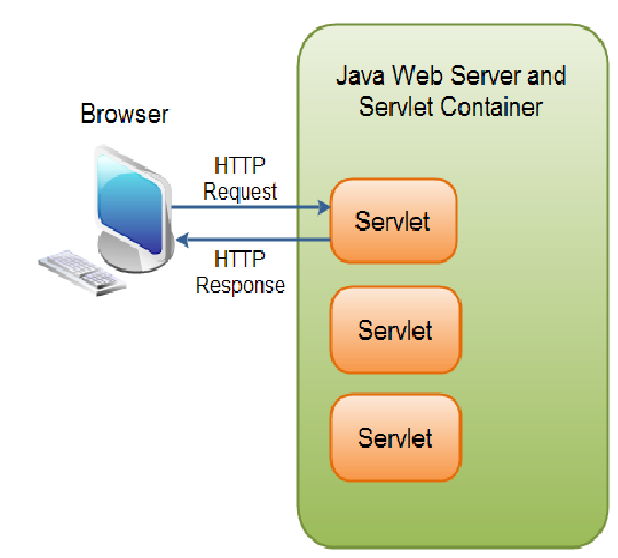
\includegraphics [scale=0.50] {servlet.png}}
  \hfill
  {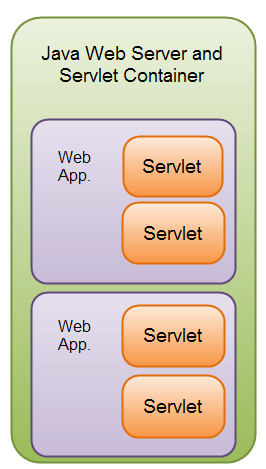
\includegraphics[scale=0.60]{servlet2.png}}
  \caption{Client Server architecture}
\end{figure}

\section{Object oriented modelling}
\subsection{Use Case Diagram}

\begin{figure}[h!]
			\centering
			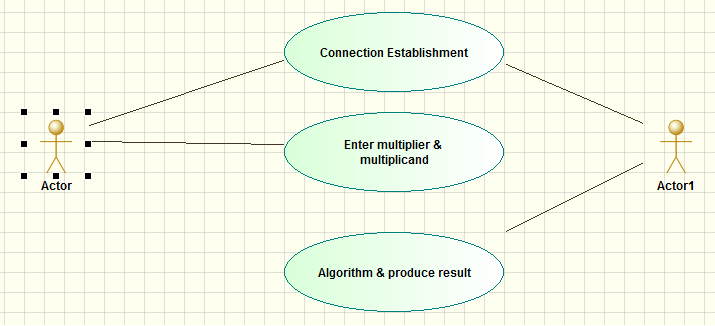
\includegraphics[scale=0.8]{usecase}
			\caption{Use case diagram}
			\label{Use case diagram}
		\end{figure}

\newpage

\subsection{Activity Diagram}

\begin{figure}[h!]
			\centering
			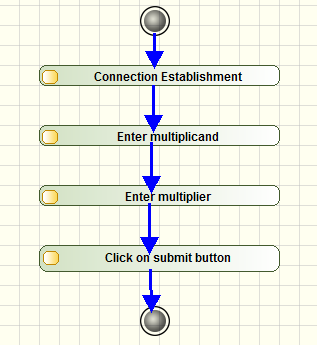
\includegraphics[scale=0.95]{activity}
			\caption{Activity diagram}
			\label{Activity diagram}
		\end{figure}


\subsection{Class Diagram}

\begin{figure}[h!]
			\centering
			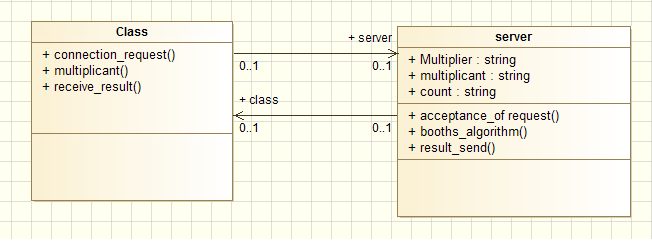
\includegraphics[scale=0.95]{class}
			\caption{Class diagram}
			\label{Class diagram}
		\end{figure}

\newpage

\section{Testing}
\subsection{BLACK BOX TESTING : }
		 Black-box testing is a method of software testing that examines the functionality of an application based on the specifications. It is also known as Specifications based testing. Independent Testing Team usually performs this type of testing during the software testing life cycle.This method of test can be applied to each and every level of software testing such as unit, integration, system and acceptance testing.\\
		 Black box testing techniques are :\\
1) Equivalence Class Partitioning\\
2) Boundary Value Analysis\\
3) Decision Tables\\
4) State Transition Diagrams (or) State Transition Diagrams\\
5) Orthogonal Arrays\\
6) All Pairs Technique\\

\subsection{WHITE BOX TESTING :}
		 White Box Testing (WBT) is also known as Code-Based Testing or Structural Testing. White box testing is the software testing method in which internal structure is being known to tester who is going to test the software.In this method of testing the testcases are calculated based on analysis internal structure of the system based on Code coverage, branches coverage, paths coverage, condition Coverage etc. Typically such method are used at Unit Testing of the code but this different as Unit testing done by the developer \& White Box Testing done by the testers, this is learning the part of the code \& finding out the weakness in the software program under test.
For tester to test the software application under test is like a white/transparent box where the inside of the box is clearly seen to the tester (as tester is aware/access of the internal structure of the code), so this method is called as White Box Testing.

The White-box testing is one of the best method to find out the errors in the software application in early stage of software development life cycle. In this process the deriving the test cases is most important part. The test case design strategy include such that all lines of the source code will be executed at least once or all available functions are executed to complete 100 percent  code coverage of testing. For this, we will use Flow Graphs. Flow graphs are, Syntactic abstraction of source code Resembling to classical flow charts Forms the basis for white box test case generation principles.Conventions of flow graph notation. \\
Why and When White-Box Testing:\\
White box testing is mainly used for detecting logical errors in the program code. It is used for
debugging a code, finding random typographical errors, and uncovering incorrect programming
assumptions .
White box testing is done at low level design and implementable code. It can be applied at all levels of
system development especially Unit, system and integration testing. White box testing can be used for
other development artefacts like requirements analysis, designing and test cases .
White box testing techniques are:\\
1. Static white box testing\\
a. Desk checking\\
b. Code walkthrough\\
c. Formal Inspections\\
2. Structural White box testing\\
a. Control flow/ Coverage testing\\
b. Basic path testing\\
c. Loop testing\\
d. Data flow \\

	\begin{figure}[h!]
		\centering
		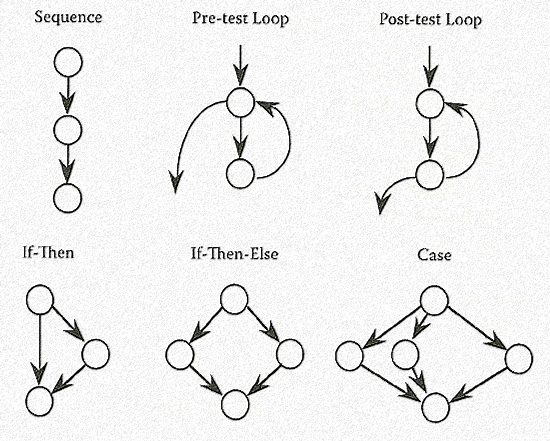
\includegraphics[scale=0.45]{CFG.png}
		\caption{Flow graph notation}
	\end{figure}

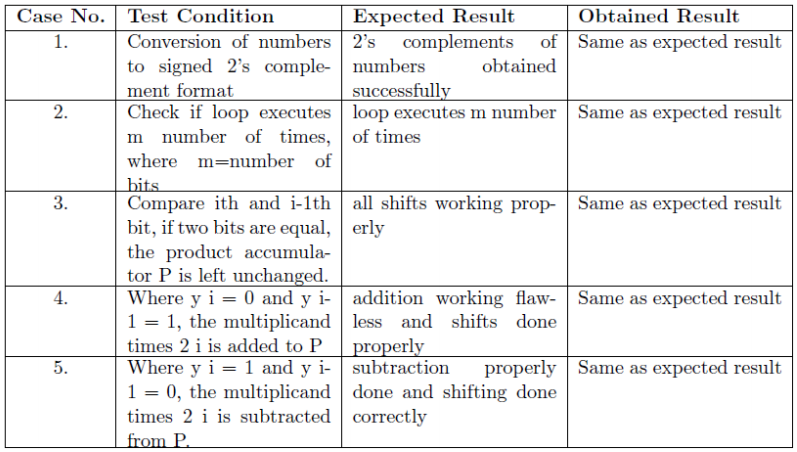
\includegraphics[width=\textwidth]{booth_whitebox}

\subsection{ POSITIVE/NEGATIVE TESTING }

\textbf{Positive Testing :}\\
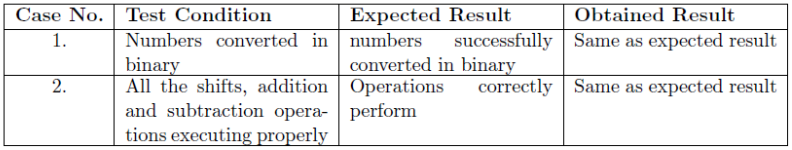
\includegraphics[width=\textwidth]{booth_positive}
\vspace{30px}

\textbf{Negative Testing :}\\
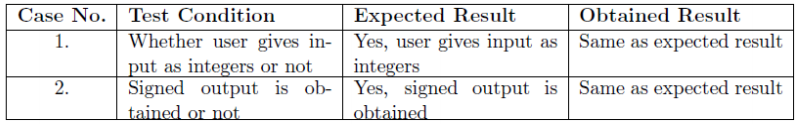
\includegraphics[width=\textwidth]{booth_negative}
\vspace{30px}


\section{Conclusion}
	\paragraph{} From this experiment, we have successfully ,used A Web Tool for Booth’s multiplication algorithm is used to multiply two numbers located in distributed environment. Use software design client-server architecture and principles for dynamic programming.
\vspace{20px}
\begin{center}
	\begin{tabular}
		{|c|c|c|c|}\hline
		{\bf Roll No.}		&{\bf Name of Student}		&{\bf Date of Performance}  				&{\bf Date of Submission}  \\ \hline
		{302}	&	{Abhinav Bakshi}& {04/01/16}		&  {25/01/16} \\ \hline
	\end{tabular}\\ 
\end{center}



\end{document}
 
